\documentclass[]{beamer}

\mode<presentation>
{
  \usetheme{Madrid}      % or try Darmstadt, Madrid, Warsaw, ...
  \usecolortheme{crane} % or try albatross, beaver, crane, ...
  \usefonttheme{default}  % or try serif, structurebold, ...
  \setbeamertemplate{navigation symbols}{}
  \setbeamertemplate{caption}[numbered]
  \setbeamercovered{transparent}
  \usefonttheme[onlymath]{serif}
} 

\usepackage[english]{babel}
\usepackage[utf8x]{inputenc}
\usepackage{mathtools, xcolor, soul, amsfonts, appendixnumberbeamer}
\graphicspath{ {images/} }


\title[Fuzzy Preference Learning]{Fuzzy Preference Learning}
\author[]{Dariush Hasanpoor}
\institute[]{Isfahan University Of Technology}
\date[]{May 24 2015}
\newcommand{\Cpl}{\emph{Preference Learning} }
\newcommand{\pl}{\emph{preference learning} }
\newcommand{\Cp}{\emph{Preference} }
\newcommand{\p}{\emph{preference} }
\newcommand{\Xtri}{$\blacktriangleright$ }
\newcommand{\Ytri}{$\triangleright$ }
\newcommand{\itemXtri}{\item[\Xtri]}
\newcommand{\itemYtri}{\item[\Ytri]}
\renewcommand{\|}[1][.3em]{\hspace{#1}|\hspace{#1}}
\renewcommand{\,}[1][.3em]{,\hspace{#1}}
\newcommand\Wider[2][3em]{%
\makebox[\linewidth][c]{%
  \begin{minipage}{\dimexpr\textwidth+#1\relax}
  \raggedright#2
  \end{minipage}%
  }%
}
\newcommand*{\Scale}[2][4]{\scalebox{#1}{$#2$}}%
\DeclarePairedDelimiter\abs{\lvert}{\rvert}%
\makeatletter
\let\oldabs\abs
\def\abs{\@ifstar{\oldabs}{\oldabs*}}
\makeatother

\definecolor{light-blue}{HTML}{66AFE9}
\definecolor{light-red}{HTML}{F77B7B}
\definecolor{light-green}{HTML}{87D13E}

\begin{document}

\begin{frame}
  \titlepage
\end{frame}

\begin{frame}{Outline}
  \tableofcontents[hideallsubsections]
\end{frame}

\section{Introduction}
\frame{\tableofcontents[currentsection]}
\subsection{What is preference?}

\begin{frame}{What is preference?}

	\begin{block}{Definition}
	\Cpl refers to the task of learning to predict an order relation on a collection of objects (alternatives).
	\end{block}
    \begin{itemize}
    \item Preference information plays a key role in automated decision making and appears in various guises in AI researches:
        \begin{itemize}
        \itemXtri Qualitative decision theory
        \itemXtri Non-monotonic reasoning
        \itemXtri Constraint satisfaction
        \itemXtri Planning
        \end{itemize}
    \end{itemize}
\end{frame}

\subsection{Notations}

\begin{frame}{Notations}
	\begin{block}{\textbf{Definition:} \textit{Weak} \Cp}
	A weak \p relation  $\succeq$ on a set $\mathcal{A}$ is a reflexive and transitive binary relation.
	\end{block}
	\pause
	\begin{block}{\textbf{Definition:} \textit{Strict} \Cp}\center
	$a \succ b  \longleftrightarrow  (a \succeq b) \wedge (b \nsucceq a)$
	\end{block}
	\pause
    \begin{itemize}
    \item In agreement with preference semantics
        \begin{itemize}
        \item[] \vspace{1em}
            \begin{table}
	            \centering
	            \begin{tabular}{c|l}
	                \textit{Notation} & \textit{Interpretation} \\\hline\rule{0pt}{1.6em}
	                $a \succeq b$ & "alternative $a$ is at least as prefered as alternative $b$." \\\rule{0pt}{1.6em}
	                $a \succ b$ & "alternative $a$ is prefered over alternative $b$."\\
	            \end{tabular}
	        \end{table}
        \end{itemize}
    \end{itemize}
\end{frame}

\begin{frame}{Preference Structure}
	\begin{block}{\textbf{Definition:} \textit{Total Strict Order (Ranking)}}\footnotesize
	If $\mathcal{A}$ is a finit set of objects/alternatives $\{a_1,\ldots,a_m\}$ a ranking of $\mathcal{A}$ can be definied with a permutation $\tau$ of $\{1,\ldots,m\}$ which {\small $a_i \succ a_j \leftrightarrow \tau(i) < \tau(j)$}.
	\end{block}
	\pause
    \begin{itemize}
    \item $\mathcal{S}_m$ is a set of all permutation of $\tau$.
    \item The task of \textit{preference learner} is to search in $\mathcal{S}_m$ space which is \emph{learning to rank}.
    \end{itemize}
\end{frame}



\subsection{Types of Ranking}

\begin{frame}{Types of Ranking}
    \begin{itemize}
    \setlength\itemsep{1em}
    \item The tasks are categorized as three main problems:\\
        \begin{itemize}
        \setlength\itemsep{.5em}
        \itemXtri \textbf{Label ranking}
        \itemXtri \textbf{Object ranking}
        \itemXtri \textbf{Instance ranking}
        \end{itemize}
    \end{itemize}
\end{frame}


\begin{frame}{Types of Ranking}{Label Ranking}
    \begin{block}{\textbf{Task}}\footnotesize
    The task of this model is to find a preference ranking among the labels for any instance.
    \end{block}
    \pause
    \vskip .4cm
    \begin{itemize}
    \item[] \textbf{Given}
        \begin{itemize}
        \setlength\itemsep{.5em}
        \item A set of training instances $\{x_k \| k = 1,\ldots,n\} \subseteq \mathcal{X}$.
        \item A set of labels $\mathcal{L} = \{\lambda_i \| i = 1,\ldots,m\}$.
        \item For each training instance $x_k$: a set of associated pairwise preferences of the form $\lambda_i \succ_{x_k} \lambda_j$.
        \end{itemize}
    \pause
    \item[] \textbf{Find}
        \begin{itemize}
        \setlength\itemsep{1em}
        \item A ranking function in the form of an $\mathcal{X} \rightarrow \mathcal{S}_m$ mapping that assigns a ranking (permutation) $\succ_x$ of $\mathcal{L}$ to every $x \in \mathcal{X}$.

        \end{itemize}
    \end{itemize}
\end{frame}

\begin{frame}{Types of Ranking}{Object Ranking}
    \begin{block}{\textbf{Task}}\small
    The task of this model is to find a preference ranking order among instances.
    \end{block}
    \pause
    \vskip .4cm
    \begin{itemize}
    \item[] \textbf{Given}
        \begin{itemize}
        \setlength\itemsep{.5em}
        \item A (potentially infinite) set X of objects (each object typically represented by a feature vector).
        \item A finite set of pairwise preferences $x_i \succ x_j$, $(x_i , x_j) \in \mathcal{X}\times\mathcal{X}$.
        \end{itemize}
    \pause
    \item[] \textbf{Find}
        \begin{itemize}
        \setlength\itemsep{1em}
        \item A ranking function that, given a set of objects $O \subset X$ as input, returns a permutation(ranking) of these objects.
        \end{itemize}
    \item<4-> In the training phase, preference learning algorithms have access to examples for which the order relation is \textbf{(partially)} known.
    \end{itemize}
\end{frame}

\begin{frame}{Types of Ranking}{Instance Ranking}
    \begin{block}{\textbf{Task}}\small
    \color{gray}{The task of this model is to find a preference ranking order among instances.}
    \end{block}
    \vskip .4cm
    \begin{itemize}
    \item[] \textbf{Given}
        \begin{itemize}
        \setlength\itemsep{.5em}
        \item \textcolor{gray}{A (potentially infinite) set X of objects (each object typically represented by a feature vector).}
        \item \textcolor{gray}{A finite set of pairwise preferences $x_i \succ x_j$, $(x_i , x_j) \in \mathcal{X}\times\mathcal{X}$.}
        \item\footnotesize An order set of labels $\mathcal{L} = \{\lambda_i \| i = 1,\ldots,m\}$ which $y_1 \succ y_2 \succ \ldots \succ y_m$.
        \item A set of $\mathcal{R} \subseteq \mathcal{X} \times \mathcal{L}$ which each instance $x_k$ is associated with a label $\lambda_{\hat{k}}$.
        \end{itemize}
    \item[] \textbf{Find}
        \begin{itemize}
        \setlength\itemsep{1em}
        \item \textcolor{gray}{A ranking function that, given a set of objects $O \subset X$ as input, returns a permutation(ranking) of these objects.}
        \end{itemize}
    \item \st{In the training phase, preference learning algorithms have access to examples for which the order relation is \textbf{(partially)} known.}
    \end{itemize}
\end{frame}


\subsection{Special Cases of preference learning}
\begin{frame}{Special Cases of preference learning}
    \begin{block}{\textbf{$\triangleright$ Classification}}
    A single class label $\lambda_i$ is assigned to each example $x_k$. This is equivalent to the set of preferences
    $\{\lambda_i \succ_{x_k} \lambda_j \| 1 \leq j \neq i \geq m\}$.    
    \end{block}
    \pause
    \vskip 1cm
    \begin{block}{\textbf{$\triangleright$ Multi-label classification}}\footnotesize
    Each training example $x_k$ is associated with a subset $\mathcal{L}_k \subseteq \mathcal{L}$ of possible labels. This is equivalent to the set of preferences 
    $\{\lambda_i \succ_{x_k} \lambda_j\|\lambda_i \in \mathcal{L}_k,\hspace{.4em}\lambda_j \in \mathcal{L} \backslash \mathcal{L}_k \}$.    
    \end{block}
\end{frame}


\section{Fuzzy Preference Learning}
\frame{\tableofcontents[currentsection]}
\subsection{Choquet Integral}
\begin{frame}{Choquet Integral}
    \onslide{An Example:}
    \begin{itemize}
    \item<1-> Suppose a school is more scientifically than literary oriented.
    \item<2-> How can we compare these 3 students?
    \item<2->[] \vspace{1em}
        \begin{table}
            \centering
            \begin{tabular}{c|ccc}
                \textit{Student} & \textit{Math} & \textit{Physics} & \textit{Literature} \\\hline
                a & 18 & 16 & 10\\
                b & 10 & 12 & 18\\
                c & 14 & 15 & 15\\
            \end{tabular}
        \end{table}\vspace{1em}
    \item<3-> A candidate set of weights can be $\{\frac{3}{8}\,\frac{3}{8}\,\frac{2}{8}\}$.
    \item<4-> But what if the school wants to favor well equilibrated students without weak points?
        \begin{itemize}
        \itemXtri Then the \textcolor{light-blue}{student \textit{c}} should be considered \textcolor{light-blue}{better than student \textit{a} and \textit{b}}.
        \itemXtri This cannot be simply done by simple \textcolor{light-red}{weighting sum} procedure!!
        \end{itemize}
    \item<5-> So how are we going rank them?!
        \begin{itemize}
        \itemXtri \textcolor{light-blue}{Choquet integral} can address such problems.
        \end{itemize}
    \end{itemize}
\end{frame}

\begin{frame}{Choquet Integral}{Continued\ldots}
    \begin{itemize}
    \itemXtri Choquet Integral
    \item[]
        \begin{align*}
        &\mathcal{C}_\mu(x) = \sum_{i = 1}^n (x_{\tau(i)} - x_{\tau(i - 1)})\mu(\{\tau(i),\ldots,\tau(n)\})\\
        &\Scale[0.8]{x_{\tau(1)}{\leq}x_{\tau(2)}\leq\ldots{\leq}x_{\tau(n)}}\,\Scale[0.8]{x_{\tau(0)} = 0}
        \end{align*}
    \end{itemize}
\end{frame}
\begin{frame}{Choquet Integral}{Continued\ldots}
    \Wider[-10cm]{
    \only<1,2>{\begin{onslide}
        \Wider[3.7cm]{\Scale[0.67]{\vbox{\begin{table}
            \centering
            \begin{tabular}{c|ccc|l|l}
                \textit{Student} & \textit{Math{\scriptsize (1)}} & \textit{Physics{\scriptsize (2)}} & \textit{Literature{\scriptsize (3)}} & \multicolumn{1}{c}{$\{\tau\}$} & \multicolumn{1}{c}{$\{x_\tau\}$}\\\hline
                a & 18 & 16 & 10 & $\{0\,3\,2\,1\}$ & $\{0\,10\,16\,18\}$\\
                b & 10 & 12 & 18 & $\{0\,1\,2\,3\}$ & $\{0\,10\,12\,18\}$\\
                c & 14 & 15 & 15 & $\{0\,1\,2\,3\}$ & $\{0\,14\,15\,15\}$\\
            \end{tabular}
        \end{table}}}}
        \vskip -.4cm
        \begin{equation*}
        \Scale[0.67]{\mathcal{C}_\mu(x) = \sum\limits_{i = 1}^{n} (x_{\tau(i)} - x_{\tau(i - 1)})\mu(\{\tau(i),\ldots,\tau(n)\})}
        \end{equation*}
        \vskip -.8cm
        \begin{align*}
        &\Scale[0.67]{\mu(\{1\,2\,3\}) = 1,}&\Scale[0.67]{\mu(\{\emptyset\}) = 0}\\
        &\Scale[0.67]{\mu(\{1\}) = \mu(\{2\}) = 0.45,}&\Scale[0.67]{\mu(\{3\}) = 0.3}\\
        &\Scale[0.67]{\mu(\{1\,3\}) = \mu(\{2\,3\}) = 0.9,}&\Scale[0.67]{\mu(\{1\,2\}) = 0.5}
        \end{align*}
    \end{onslide}}
    \only<3>{\begin{onslide}
        \Wider[7cm]{\Scale[0.67]{\vbox{\begin{table}
            \centering
            \begin{tabular}{c|ccc|cc}
                \textit{Student} & \textit{Math} & \textit{Physics} & \textit{Literature} & \textcolor{light-red}{Weighted sum} & \textcolor{light-green}{Choquet integral}\\\hline
                a & 18 & 16 & 10 & \textcolor{light-red}{15.25} & \textcolor{light-green}{13.9}\\
                b & 10 & 12 & 18 & \textcolor{light-red}{12.75} & \textcolor{light-green}{13.6}\\
                c & 14 & 15 & 15 & \textcolor{light-red}{14.62} & \textcolor{light-green}{14.9}\\
            \end{tabular}
        \end{table}}}}
    \end{onslide}}}
    \vskip -.7cm
    \only<2>{\begin{onslide}
    \Wider[-3cm]{\Scale[0.68]{\vbox{
    \begin{align*}
    &\mathcal{C}_\mu(a) = (10 - 0) \times \mu(\{3,2,1\}) + (16 - 10) \times \mu(\{2,1\}) + (18 - 16) \times \mu(\{1\}) = 13.9\\
    &\mathcal{C}_\mu(b) = (10 - 0) \times \mu(\{1,2,3\}) + (12 - 10) \times \mu(\{2,3\}) + (18 - 12) \times \mu(\{3\}) = 13.6\\
    &\mathcal{C}_\mu(c) = (14 - 0) \times \mu(\{3,2,1\}) + (15 - 14) \times \mu(\{2,3\}) + (15 - 15) \times \mu(\{3\}) = 14.9
    \end{align*}}}}
    \end{onslide}}
\end{frame}

\begin{frame}{Non-additive Measures}
    \begin{itemize}
    \item As in previous example, we had \textcolor{light-blue}{$\Scale[0.8]{\mu(\{1\}) = \mu(\{2\}) = 0.45}\,\Scale[0.8]{\mu(\{1\,2\}) = 0.5}$}.
    \item[] 
        \begin{itemize}
        \itemXtri We can see \textcolor{light-blue}{$\Scale[0.8]{\mu(\{1\,2\}) \neq \mu(\{1\}) + \mu(\{2\})}$}.
        \end{itemize}
    \end{itemize}
    \pause
    \begin{block}{\textbf{Definition:} Non-additive(Capacities) Measures}
        Let $\mathcal{X} = \{x_1\,\ldots\,x_n\}$ be a finit set and $\mu$ a measure $2^\mathcal{X} \rightarrow [0\,1]$ if there are $A\,B \subseteq \mathcal{X}\|A \cap B = \emptyset$ such that $\mu(\{A, B\}) \neq \mu(\{A\}) + \mu(\{B\})$ then the measure $\mu$ is a non-additive or capacity fuzzy measure.
    \end{block}
    \pause
    \begin{itemize}
    \itemXtri Non-additive measures are normalized and monotone.\vspace{.5em}
        \Wider[.0cm]{\Scale[0.9]{\vbox{\begin{itemize}
        \item[] $\mu(\emptyset) = 0\, \mu(\mathcal{X}) = 1$ and\vspace{.2em}
        \item[] $\mu(A) \leq \mu(B)\hspace{1em}\forall\hspace{.2em}A \subseteq B \subseteq \mathcal{X}$
        \end{itemize}}}}
    \itemXtri \textcolor{light-blue}{Choquet Integral} combines non-additive measures in a desirable way.
    \end{itemize}
\end{frame}

\begin{frame}{Non-additive Measures}{M$\mathrm{\ddot{o}}$bius transform}
    \only<1,2>{\begin{block}{\textbf{Definition:} M$\mathrm{\ddot{o}}$bius transform}
    \begin{align*}
    &\mu(B) = \sum_{A \subseteq B} m(A)\\
    &m_{\hat{\mu}}(A) = \sum_{v \subseteq A} (-1)^{\abs{A} - \abs{v}}\hat{\mu}(v)
    \end{align*}
    \end{block}}
    \pause
    \only<2,3>{\begin{block}{Example}\scriptsize
    \begin{align*}
    &m_{\hat{\mu}}(\{\emptyset\}) = \hat{\mu}(\emptyset)\\
    &m_{\hat{\mu}}(\{1\}) = \hat{\mu}(\{1\}) - \hat{\mu}(\emptyset)\\
    &m_{\hat{\mu}}(\{1, 2\}) = \hat{\mu}(\{1, 2\}) - \hat{\mu}(\{1\}) - \hat{\mu}(\{2\}) + \hat{\mu}(\emptyset)\\
    \end{align*}
    \end{block}}
    \pause
    \only<3>{\begin{itemize}\footnotesize
    \itemXtri The value $m_{\hat{\mu}}(A)$ can be interpreted as the weight that is exclusively allocated to $A$, instead of being indirectly connected with $A$ through the interaction with other subsets.
    \end{itemize}}
\end{frame}

\subsection{Fuzzy Preference Learning Using Choquet Integral}
\begin{frame}{Fuzzy Preference Learning Using Choquet Integral}
    \begin{itemize}[<+->]
    \setlength\itemsep{1em}
    \itemXtri Suppose that $f: \mathcal{X} \rightarrow \mathbb{R}_{+}$ is any nonnegative function that assigns a \emph{value} to each criterion $x_i$ for any object.
    \itemXtri \textbf{Question:} How to aggregate the evaluations of individual criteria?
    \itemXtri \textbf{Answer:} This overall evaluation can be considered as an integral $\mathcal{C}_{\mu}(f)$ of the function $f$ with respect to the measure $\mu$.
    \itemXtri This article has focued on \textcolor{light-blue}{object ranking} problem.
    \end{itemize}
\end{frame}

\begin{frame}{Fuzzy Preference Learning Using Choquet Integral}{Continued\ldots}
    \begin{align*}
        \mathcal{C}_{\hat{\mu}}(f) &= \sum_{i = 1}^{n}(f(x_{(i)}) - f(x_{(i - 1)}))\cdot\mu(\overbrace{\{x_{(i)}\,\ldots\,x_{(n)}\}}^{A_{(i)}})\\
        &= \sum_{i = 1}^{n}f(x_{(i)})\cdot(\mu(A_{(i)}) - \mu(A_{(i+1)}))\\
        &\stackrel{\mathclap{\normalfont\mbox{{\tiny MT}}}}{=} \sum_{i = 1}^{n}f(x_{(i)})\cdot\sum_{R \subseteq \mathcal{T}} m(R)\|\Scale[0.78]{\mathcal{T} = \big\{\mathcal{G} \cup \{x_{(i)}\}\|\mathcal{G} \subset \{x_{(i+1)}\,\ldots\,x_{(n)}\}\big\}}\\
        &= \sum_{T \subseteq \mathcal{X}} m(T) \times \min_{x_i \in T}f(x_i)\\
        &= \sum_{T \subseteq \mathcal{X}} \sum_{v \subseteq T} (-1)^{\abs{A} - \abs{v}}\hat{\mu}(v) \times \min_{x_i \in T}f(x_i)
    \end{align*}
\end{frame}


\begin{frame}{Fuzzy Preference Learning Using Choquet Integral}{Continued\ldots}
    \begin{block}{Description of approach}
    \begin{itemize}\footnotesize
    \setlength\itemsep{.7em}
    \itemXtri Training data to be available in the form of a set of objects $o_i$.
    \itemXtri Every object $o_i$ is linked to a corresponding label information $l_i$.
    \itemXtri A set $\mathcal{D}$ is constructed: $(o_i\,o_j) \in \mathcal{D}$ suggesting that $o_i \succ o_j \| l_i > l_j$.
    \itemXtri The \textcolor{light-blue}{Choquet integral} is uniquely identified by the underlying measure $\mu$ on the set of criteria $\mathcal{X}$, the problem comes down to defining $\mu$.
    \itemXtri Finding $\mu$ measure is actually a optimization problem!
    \end{itemize}
    \end{block}
\end{frame}
\subsection{Results}
\begin{frame}{Experiments}{Datebases}
    \begin{figure}
        \centering
        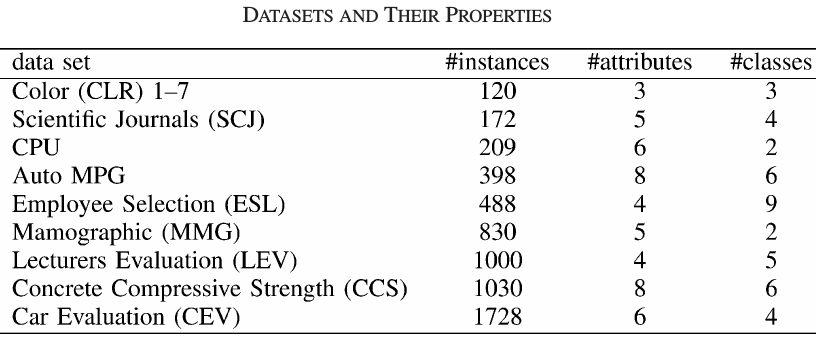
\includegraphics[width=.8\textwidth]{db}
    \end{figure}
\end{frame}
\begin{frame}{Experiments}{Results}
    \begin{figure}
        \centering
        \only<1>{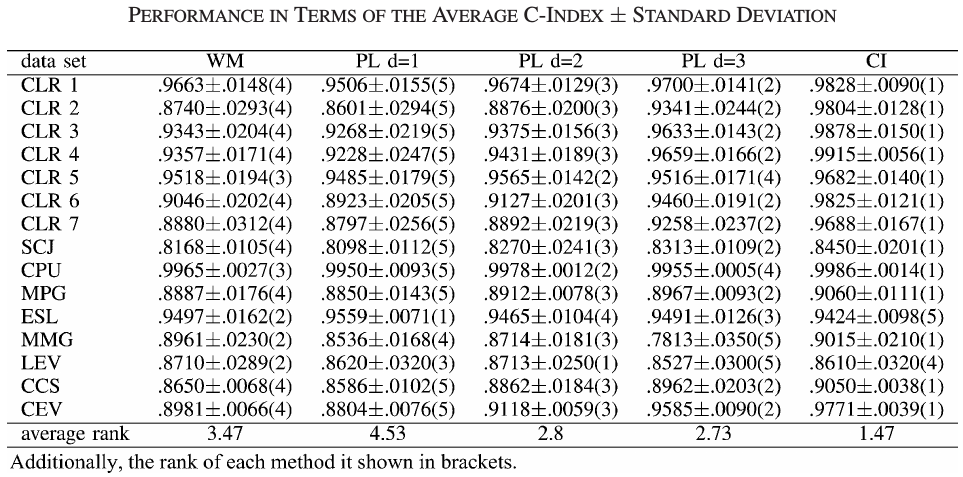
\includegraphics[width=.9\textwidth]{results}}
        \only<2>{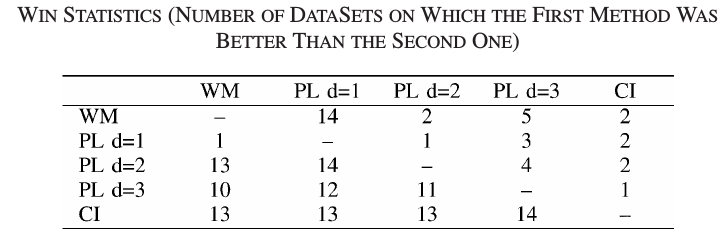
\includegraphics[scale=.4]{results_2}}
    \end{figure}
    \begin{itemize}
    \item[] Compared the approach with kernel-based methods.
        \begin{itemize}
            \itemXtri Spider implementation of the RankSVM approach with a linear and a polynomial kernel(PL) with kernel degree of $d$.
            \itemXtri Weighted Mean(WM). 
    \end{itemize}         
    \end{itemize}
\end{frame}
\section{References}
\begin{frame}{References}
    \nocite{*}
    {\scriptsize
    \bibliographystyle{IEEEtran}
    \bibliography{reference}
    }
\end{frame}

\appendix

\section{Techniques}
\frame{\tableofcontents[currentsection]}
\subsection{Learning Utility Function}
\begin{frame}{Techniques}{Learning Utility Function}
    \begin{itemize}
    \item A natural way to represent preferences is to evaluate the alternatives by means of a utility function.
    \end{itemize}
    \pause
    \begin{block}{\textbf{Object Preferences Senario}}
        \begin{itemize}[<+->]
        \itemYtri Such a function is a mapping $\mathcal{F} : \mathcal{X} \rightarrow \mathcal{U}$ that assigns a utility degree $\mathcal{F}(x)$ to each object $x$ and, thereby, induces a linear order on $\mathcal{X}$.
        \end{itemize}
    \end{block}
    \begin{block}{\textbf{Label Preferences Senario}}
        \begin{itemize}[<+->]
        \itemYtri A utility function $\mathcal{F}_i : \mathcal{X} \rightarrow \mathcal{U}$ is needed for every label $\lambda_i , i = ,\ldots,m$.
        \itemYtri $\mathcal{F}(x)$ is the utility assigned to alternative $\lambda_i$ by instance $x$.
        \itemYtri A ranking $\succ_x$ is derived that satisfies $\lambda_i \succ_x \lambda_j \rightarrow \mathcal{F}_i(x)\geq\mathcal{F}_j(x)$.
        \end{itemize}
    \end{block}
\end{frame}
\subsection{Learning Preference Relations}
\begin{frame}{Techniques}{Learning Preference Relations}
    \begin{itemize}\footnotesize
    \item  An alternative approach to preference learning consists of comparing pairs of objects(labels) in terms of a binary preference relation.
    \end{itemize}
    \pause
    \begin{block}{\textbf{Object Preferences Senario}}\footnotesize
        \begin{itemize}[<+->]
        \itemYtri Learning a binary preference predicate $\mathcal{Q}(x, x')$, which
predicts whether $x$ is preferred to $x'$ or vice versa.
        \itemYtri A final ordering is found in a second phase by deriving a ranking that is maximally consistent with these predictions.
        \end{itemize}
    \end{block}
    \begin{block}{\textbf{Label Preferences Senario}}\scriptsize
        \begin{itemize}[<+->]
        \itemYtri One can train a separate model(base learner) $\mathcal{M}_{i,j}$ for each pair of labels $(\lambda_i , \lambda_j ) \in \mathcal{L},\hspace{.5em}1\leq i < j \leq m$; thus, a total number of $\frac{m(m - 1)}{2}$ models is needed.
        \itemYtri  For training, a preference information of the form $\lambda_i \succ_x \lambda_j$ is turned into a (classification) example $(x, y)$ for the learner $\mathcal{M}_{a,b}$, where $a = \min(i, j)$ and $b = \max(i, j)$.
        \itemYtri $\mathcal{M}_{a,b}$ is intended to learn the mapping that outputs 1 if $\lambda_a \succ_x \lambda_b$ and 0 if $\lambda_b \succ_x \lambda_a$.
        \end{itemize}
    \end{block}
\end{frame}

\section{Fuzzy Preference Learning}
\frame{\tableofcontents[currentsection]}
\begin{frame}{Fuzzy Preference Learning Using Choquet Integral}{Continued\ldots}
    \begin{itemize}[<+->]
    \setlength\itemsep{.5em}
    \itemXtri The idea is to represent the latent utility function $\mathcal{U}(\cdot)$ in terms of a Choquet integral.
    \itemXtri Assuming that objects $o \in \mathcal{O}$ are represented as feature vectors:
    \item[]<2->\hspace{7em}$f_o = (f_o(x_1)\,\ldots\,f_o(x_n))$
    \itemXtri $f_o(x_i)$ can be thought of as the evaluation of object $o$ on the criterion $x_i$, So:
    \item[]<3->\hspace{10em}$\mathcal{U}(o) = \mathcal{C}_{\mu}(f_o)$
    \itemXtri The goal is to minimizes the number of ranking errors($\mathcal{C}$-index) on the training data $\mathcal{D}$.
    \item[]<4->\hspace{4em}$C(U,O) = \frac{\sum\limits_{1{\leq}i<j{\leq}k}\hspace{.3em}\sum\limits_{(o,o\prime) \in O_i \times O_j}\mathcal{S}(\mathcal{U}(o)\,\mathcal{U}(o\prime))}{\sum\limits_{i<j}\abs{O_i}.\abs{O_j}}\,\mathcal{S}(u,v) = \begin{cases}1 & u < v\\0 & \text{otherwise}\end{cases}$
    \end{itemize}
\end{frame}

\end{document}